\documentclass[
  11pt,
  letterpaper,
   addpoints,
   answers
  ]{exam}

\usepackage{../exercise-preamble}
\usepackage{float}
\usepackage[most]{tcolorbox}

\begin{document}

\noindent
\begin{minipage}{0.47\textwidth}

\includegraphics[width=\textwidth]{../fcfm_die}
\end{minipage}
\begin{minipage}{0.53\textwidth}
\begin{center} 
\large\textbf{Análisis de Sistemas Dinámicos y Estimación} (EL3204-1) \\
\large\textbf{Control 1} \\
\normalsize Prof.~ Marcos Orchard - Sebastián Espinosa.\\
\normalsize Prof.~Aux.~Erik Sáez
\end{center}
\end{minipage}

\begin{tcolorbox}[colback=yellow!10!white,colframe=black!80!white,title=Instrucciones]
Dispone de 2 horas para contestar el control. No se permite el uso de calculadoras ni teléfonos. Recuerde escribir su nombre en todas las hojas. La sospecha de copia será sancionada.
\end{tcolorbox}

\begin{questions}
  %%%%%%%%%%%%%%%%%%%%%%%%%%%
  \question

Se requiere estudiar la velocidad y posición que tendrá el sistema de amortiguamiento para un vehículo que será enviado a la luna dada determinadas características.
Para ello, tenga en cuenta que se conoce la masa $m$ del vehículo, la constante de amortiguamiento $c$ y la longitud de onda promedio de la superficie lunar $L$ de la zona donde se encuentra.
  Además, considere que el suelo lunar se puede modelar por $y(t) = a \cos\left(\frac{2\pi s(t)}{L}\right)$, donde $s(t)$ es la distancia recorrida por el vehículo.

% --- Espacio para la figura del enunciado ---
\begin{figure}[H]
  \centering
  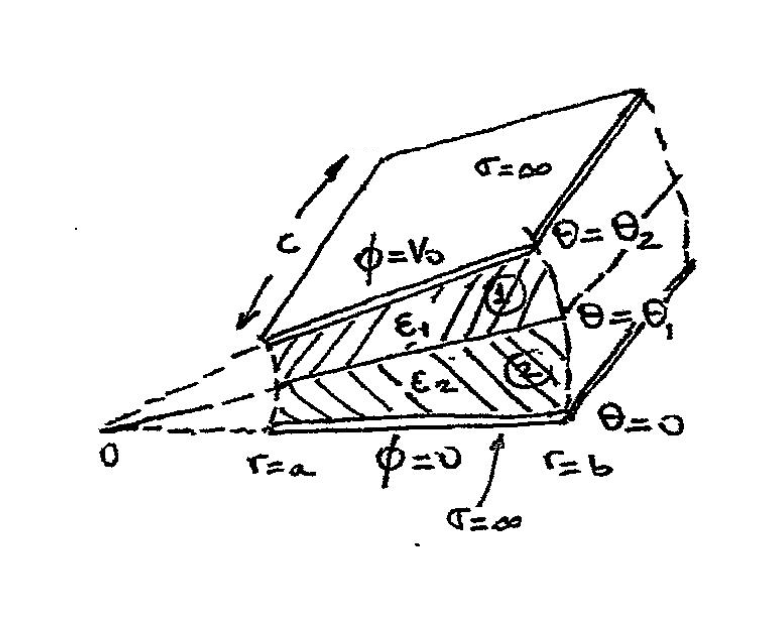
\includegraphics[width=0.7\textwidth]{Control_1_1} % Descomenta y pon el nombre correcto de la imagen
  \caption{A la izquierda se encuentra la posición de equilibrio y la segunda en movimiento del modelo de sistema masa-resorte-amortiguador sobre superficie lunar.}
  \label{fig:modelo_luna}
\end{figure}

\begin{figure}[H]
  \centering
  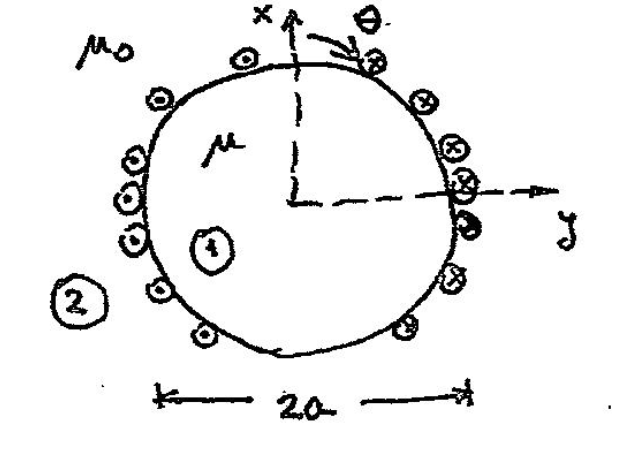
\includegraphics[width=0.5\textwidth]{Control_1_2} % Cambia el nombre si es necesario
  \caption{Perfil de la superficie lunar modelada como función cosenoidal.}
  \label{fig:superficie_lunar}
\end{figure}

\begin{enumerate}
  \item \textbf{[1 punto]} Establezca las hipótesis simplificatorias que sean necesarias. 
  \item \textbf{[2 puntos]} Encuentre la EDO que modela este sistema considerando que el amortiguador es de un tipo especial tal que es proporcional al cuadrado de la velocidad de la masa acoplada.

  \item \textbf{[1.5 puntos]} Reescriba el sistema de forma matricial, además encuentre estados cero, equilibrio y tierra (en caso de existir).

  \item \textbf{[1 punto]} Linealice en torno a un punto de operación arbitrario ($\vec{X}(t), u(t)$). Donde $\vec{X}(t)$ corresponde al vector de estados y $u(t)$ a la variable de entrada.

  \item \textbf{[0.5 puntos]} Del paso anterior, señale el vector de estados, la matriz de estados, la matriz de entrada, la variable de entrada y la variable de salida.

\end{enumerate}

%--------------------------
\begin{solution}
\subsection*{Resolución 1.1}
Las siguientes hipótesis simplificatorias se consideran razonables para el modelo:
\begin{itemize}
  \item La masa $m$ del vehículo es constante y se considera concentrada en un solo punto (modelo de partícula).
  \item El resorte tiene constante elástica $k$ y cumple la ley de Hooke en todo el rango de operación.
  \item El amortiguador tiene una fuerza proporcional al cuadrado de la velocidad, es decir, $F_c = c \dot{x}^2$ (según lo indicado en el enunciado).
  \item El contacto entre la rueda y la superficie lunar es perfecto, es decir, no hay deslizamiento ni pérdidas por fricción adicionales.
  \item La superficie lunar se modela como una función cosenoidal conocida y no cambia con el tiempo.
  \item Se desprecia la resistencia del aire y cualquier otra fuerza externa distinta a las consideradas.
  \item El movimiento se considera unidimensional a lo largo de la dirección $s$.
  \item Los parámetros $m$, $c$, $k$, $a$ y $L$ son constantes y conocidos.
  \item \dots
\end{itemize}

\subsection*{Resolución 1.2}

Para modelar el movimiento del centro de masa $x$ del vehículo respecto al suelo $y$, aplicamos la segunda ley de Newton considerando todas las fuerzas relevantes:
\begin{itemize}
  \item \textbf{Fuerza del resorte:} $-k(x - y)$, donde $x$ es la posición de la masa y $y$ la posición de la superficie lunar bajo la rueda.
  \item \textbf{Fuerza del amortiguador no lineal:} $-c\dot{x}^2$, proporcional al cuadrado de la velocidad.
\end{itemize}

La ecuación de movimiento es:
\begin{align}
  m\ddot{x} &= -k(x - y) - c\dot{x}^2\\
  m\ddot{x} &= -kx + ky - c\dot{x}^2 \\
  m\ddot{x} + c\dot{x}^2 + kx &= ky
\end{align}

Dado que la superficie lunar se modela como
\begin{equation}
  y(t) = a\cos\left(\frac{2\pi s(t)}{L}\right)
\end{equation}
y si el vehículo avanza a velocidad constante $v$, entonces $s(t) = vt$ y por lo tanto:
\begin{equation}
  y(t) = a\cos\left(\frac{2\pi v t}{L}\right)
\end{equation}

Las condiciones iniciales, para generalidad, pueden ser:
\begin{align}
  \dot{x}(0) &= x_0 \\
  x(0) - y(0) &= l_0
\end{align}
Si el vehículo parte en $t=0$ sobre un máximo de la superficie ($y(t=0) =a\cos(0) = a$), entonces:
\begin{align}
  x(0) - a &= l_0 \implies x(0) = l_0 + a
\end{align}

Por lo tanto, la ecuación diferencial final que modela el sistema es:
\begin{equation}
  \boxed{
    \ddot{x}(t) + \frac{c}{m} \dot{x}^2(t) + \frac{k}{m} x(t) = \frac{k}{m} y(t)
  }
\end{equation}
donde $y(t) = a\cos\left(\frac{2\pi v t}{L}\right)$, con condiciones iniciales $x(0) = l_0 + a$ y $\dot{x}(0) = x_0$.

Esta ecuación describe la dinámica del sistema masa-resorte-amortiguador sobre la superficie lunar modelada, considerando la no linealidad del amortiguador y la excitación periódica del terreno.

\subsection*{Resolución 1.3}


Dado que identificamos que el sistema sera no lineal:
\begin{equation}
  \ddot{x}(t) + \frac{c}{m} \dot{x}^2(t) + \frac{k}{m} x(t) = \frac{k}{m} y(t)
\end{equation}
Como la variable que estamos analizando es $\ddot{x}$ luego el vector de estados sera:
\begin{equation}
  \vec{X}(t) = \begin{pmatrix} x(t) \\ \dot{x}(t) \end{pmatrix}
\end{equation}
El sistema se puede escribir como:
\begin{equation}
  \dot{\vec{X}}(t) = \begin{pmatrix} \dot{x}(t) \\ -\frac{c}{m} \dot{x}^2(t) - \frac{k}{m} x(t) + \frac{k}{m} y(t) \end{pmatrix}
\end{equation}
Donde la salida es:
\begin{equation}
  \vec{Y}(t) = \begin{pmatrix} 1 & 0 \\ 0 & 1 \end{pmatrix} \vec{X}(t)
\end{equation}
Luego queremos analizar los diferentes estados, por lo que tenemos lo siguiente:
\begin{itemize}
    \item \textbf{Estado cero:} El estado cero es aquel para el cual, con entrada y condiciones iniciales nulas, la salida es cero:
\begin{equation}
  \vec{X}_0 = \begin{pmatrix} 0 \\ 0 \end{pmatrix}
\end{equation}

\item \textbf{Estado tierra:} El estado tierra es el estado al que el sistema converge para entrada nula y cualquier condición inicial, si existe. En este caso, si el carro no puede bajar más allá del largo natural del resorte (por ejemplo, $l_0$), entonces:
\begin{equation}
  \vec{X}_t = \begin{pmatrix} 0 \\ 0 \end{pmatrix}
\end{equation}
	\item \textbf{Estado de equilibrio:} El estado de equilibrio $\vec{X}_e$ es aquel para el cual $\dot{\vec{X}}(t) = \vec{0}$ con entrada nula. Imponiendo esta condición:
\begin{align}
  \dot{\vec{X}}_e &= \begin{pmatrix} \dot{x}_e \\ -\frac{c}{m} \dot{x}_e^2 - \frac{k}{m} x_e \end{pmatrix} = \begin{pmatrix} 0 \\ 0 \end{pmatrix}
\end{align}
De la primera ecuación, $\dot{x}_e = 0$. De la segunda, $0 = -\frac{k}{m} x_e$ implica $x_e = 0$.
Por lo tanto,
\begin{equation}
  \vec{X}_e = \begin{pmatrix} 0 \\ 0 \end{pmatrix}
\end{equation}
\end{itemize}
Así, los tres estados especiales coinciden en este sistema bajo entrada nula y con las hipótesis dadas.

\subsection*{Resolución 1.4}

Para linealizar el sistema en torno a un punto de operación arbitrario $\left(\vec{X}_p, y_p\right)$, usamos la expansión de Taylor de primer orden:
\begin{align}
  \dot{\vec{X}}(t) &\approx f(\vec{X}_p, y_p) + \left.\frac{\partial f}{\partial \vec{X}}\right|_{\vec{X}_p, y_p} (\vec{X}(t) - \vec{X}_p) + \left.\frac{\partial f}{\partial y}\right|_{\vec{X}_p, y_p} (y(t) - y_p)
\end{align}

Dado el sistema:
\begin{equation}
  \dot{\vec{X}}(t) = \begin{pmatrix} \dot{x}(t) \\ -\frac{c}{m} \dot{x}^2(t) - \frac{k}{m} x(t) + \frac{k}{m} y(t) \end{pmatrix}
\end{equation}

Calculamos las derivadas parciales:
\begin{align}
  \frac{\partial f}{\partial \vec{X}} =
  \begin{pmatrix}
    \frac{\partial \dot{x}(t)}{\partial x(t)} & \frac{\partial \dot{x}(t)}{\partial \dot{x}(t)} \\
    \frac{\partial}{\partial x(t)}\left(-\frac{c}{m} \dot{x}^2(t) - \frac{k}{m} x(t) + \frac{k}{m} y(t)\right) & \frac{\partial}{\partial \dot{x}(t)}\left(-\frac{c}{m} \dot{x}^2(t) - \frac{k}{m} x(t) + \frac{k}{m} y(t)\right)
  \end{pmatrix}
\end{align}

Evaluando en el punto de operación $\left(\vec{X}_p, y_p\right)$:
\begin{align}
  \left.\frac{\partial f}{\partial \vec{X}}\right|_{\vec{X}_p, y_p} =
  \begin{pmatrix}
    0 & 1 \\
    -\frac{k}{m} & -\frac{2c}{m} \dot{x}_p
  \end{pmatrix}
\end{align}

La derivada parcial respecto a $y(t)$ es:
\begin{align}
  \left.\frac{\partial f}{\partial y}\right|_{\vec{X}_p, y_p} = \begin{pmatrix} 0 \\ \frac{k}{m} \end{pmatrix}
\end{align}

Por lo tanto, el sistema linealizado alrededor del punto de operación $\left(\vec{X}_p, y_p\right)$ se expresa como:
\begin{align}
  \dot{\vec{X}}(t) &\approx f(\vec{X}_p, y_p) +
  \begin{pmatrix}
    0 & 1 \\
    -\frac{k}{m} & -\frac{2c}{m} \dot{x}_p
  \end{pmatrix}
  (\vec{X}(t) - \vec{X}_p) +
  \begin{pmatrix} 0 \\ \frac{k}{m} \end{pmatrix} (y(t) - y_p)
\end{align}

\subsection*{Resolución 1.5}

A partir de la linealización realizada, identificamos los siguientes elementos del sistema en espacio de estados:

\begin{itemize}
  \item \textbf{Vector de estados:}
  \begin{equation}
    \vec{X}(t) = \begin{pmatrix} x(t) \\ \dot{x}(t) \end{pmatrix}
  \end{equation}
  \item \textbf{Matriz de estados (evaluada en el punto de operación $\vec{X}_p$):}
  \begin{equation}
    A = \begin{pmatrix} 0 & 1 \\ -\frac{k}{m} & -\frac{2c}{m} \dot{x}_p \end{pmatrix}
  \end{equation}
  \item \textbf{Matriz de entrada:}
  \begin{equation}
    B = \begin{pmatrix} 0 \\ \frac{k}{m} \end{pmatrix}
  \end{equation}
  \item \textbf{Variable de entrada:}
  \begin{equation}
    u(t) = y(t)
  \end{equation}
  \item \textbf{Matriz de salida:}
  \begin{equation}
    C = \begin{pmatrix} 1 & 0 \\ 0 & 1 \end{pmatrix}
  \end{equation}
  \item \textbf{Variable de salida:}
  \begin{equation}
    \vec{Y}(t) = C \vec{X}(t)
  \end{equation}
\end{itemize}

Así, el sistema linealizado queda completamente caracterizado en términos de sus matrices y variables principales.
\end{solution}

\end{questions}
\end{document}